\documentclass[12pt]{article} %正文字体大小为小四
\usepackage{ctex}
\usepackage{import}
\usepackage{hyperref}	% 用于交叉引用
\usepackage{setspace}	% 用于设置行间距
\usepackage{listings}	% 用于代码高亮
\usepackage{xcolor}		% 用于处理颜色
\usepackage{ulem}		% 用于各种线
\usepackage{amsmath}	% 用于数学公式(如 \begin{align})
\usepackage{amsthm}		% 用于数学版式(如 \newtheorem{cmd}{caption})
\usepackage{booktabs}	% 用于表格画线
\usepackage{graphicx}	% 用于插入图片
%\usepackage{minted}
\usepackage{cite} %Bibtex引用
\usepackage{amssymb}
\usepackage{tabularx}
\usepackage{tikz}
\usetikzlibrary{arrows}
\usepackage{graphviz}


\usepackage{makecell}
\usepackage{boldline}

\usepackage{algorithm}
\usepackage{algorithmicx}
\usepackage{algpseudocode}
\usepackage{amsmath}

% 用于伪代码
\floatname{algorithm}{算法}
\renewcommand{\algorithmicrequire}{\textbf{输入:}}
\renewcommand{\algorithmicensure}{\textbf{输出:}}

% 用于表格粗线部分
\makeatletter
\def\hlinewd#1{
\noalign{\ifnum0=`}\fi\hrule \@height #1
\futurelet\reserved@a\@xhline}
\makeatother

% tikz 样式
\tikzset{
    treenode/.style={align=center,inner sep=0pt,text centered,circle,minimum width=25pt,minimum height=25pt},
    bluenode/.style={treenode,draw=blue},
    rednode/.style={treenode,draw=red},
    blacknode/.style={treenode,draw=black},
    caption/.style={below=0.3cm, align=flush center,text width=8cm},
    abovecaption/.style={above=0.3cm, align=flush center,text width=8cm}
    level 1/.style = {sibling distance=3cm},
    level 2/.style = {sibling distance=2cm},
    level 3/.style = {sibling distance=2cm}, 
    level distance = 2.5cm
}

\usepackage[top = 0.8in, bottom = 0.8in, left = 0.8in, right = 0.8in]{geometry} %设置页边距
%按照老师标准修改格式

%首行缩进2字符
\RequirePackage{indentfirst}
\setlength{\parindent}{2em}
% 行间距1.15
\linespread{1.15}


\title{研究性学习结题报告书}


\author{}
\begin{document}
	
\maketitle

\begin{itemize}
	\item[\textbf{课题名称}] 用信息方法研究遗传学问题 \centering
	\item[\textbf{课题负责人}] 杨景云
	\item[\textbf{课题成员}] blablabla
	\item[\textbf{指导教师}] 李丽华老师
	\item[\textbf{所在班级}] 高二(9)班
\end{itemize}

\newpage 

\begin{abstract}
\fontsize{12.0pt}{\baselineskip}\selectfont %小四
%\newline %空一行
高中生物中有关基因遗传的计算问题一直是学习中的难点。本文从高中生物中的常见问题切入,建立一个计算遗传学中表现型比例,基因型比例和最优杂交方案的数学模型并提出了高效求解该模型的算法。本文通过对基因片段二进制编码后, 引入集合幂级数来表示基因片段出现次数。根据遗传学基本定律,产生配子和配子结合的过程就是集合幂级数的不同形式卷积。进而用快速莫比乌斯变换和快速沃尔什变换算法在很低的算法时间复杂度内求解该问题。
该模型得出了手工求解表现型和基因型比例的通用方法,以及基于用计算机高效求解的算法。文章最后,根据此模型求解了实际应用中的若干个问题。
\newline %空一行
\newline
\textbf{关键字:}
\newline %空一行
\end{abstract}

\newpage

\tableofcontents % 目录,需编译两次

\newpage

\section{引言}

高中生物中的遗传学问题一直是学习中的难点。由于缺少既高效又通用的方法,很容易在复杂的表现型比例,基因型比例的计算中出错。同时,在设计杂交方案等具有综合性的问题中也会遇到困难。而本文试图通过引入如生成函数等更高级的数学工具,以及计算机方法来探索新的求解方法。

我们提出的数学建模思路来源于一个出现在教辅书上的经典问题\cite{蔡雪燕2009浅谈高中生物概念教学}: 基因型为$\text{AaBB}$的个体自交,但含有$\text{a}$基因的个体有 $\frac{1}{2} $ 的几率不能存活。给出的解法\cite{张克芳2013浅析高中生物遗传学习题的解析技巧}:含有A基因的配子的概率为$2/3$,含有a基因的配子的概率为$1/3$。如果把不同配子看成多项式的系数,基因型看做指数,那么杂交过程就可以看成多项式乘法. 
$(\frac{2}{3}x^{\text{A}}+\frac{1}{3} x^{\text{a}})((\frac{1}{2}x^{\text{B}}+\frac{1}{2}x^{\text{B}})=2\frac{2}{3}x^{\text{AB}}+\frac{1}{3}x^{\text{aB}}$ 那么两种基因型的比例就是$2:1$. 这种方法将生物学问题转化成纯粹的数学问题,但引入算式的部分缺乏严谨性。本文将运用这种方法的思想,将这种算式抽象化为集合幂级数。通过将$\text{AB}$这样的基因集合定义为广义的指数,将模型在数学上严格化,进而得到通用的手工求解做法。

更重要的是,随着基因片段长度的增加,这种方法计算的复杂度会大大增加。这时我们就可以引入计算机手段来求解该问题。如果直接模拟多项式的乘法过程,算法时间复杂度依然很高。此时就需要运用能求解集合幂级数卷积的高效算法:快速沃尔什变换(Fast Walsh Transform,FWT)和快速莫比乌斯变换(Fast Mobius Transform,FMT)。


\section{文献综述}

19世纪末,遗传学的基本定律已经由孟德尔(Gregor Johann Mendel),摩尔根(Thomas Hunt Morgan)等人提出,并在细胞学研究中证明。基因的分离定律(Law of Segregation)和自由组合定律(Free Combination Law of Gene Independent Assortment)使得遗传学中的出现频率问题可以用组合数学计算。\cite{2009陈阅增普通生物学}

作为组合数学的高效工具,生成函数(Generating Function,又称母函数)最初由棣莫弗(Abraham De Moivre)提出,最初是用于求线性递推数列的通项公式。\cite{knuth2005art}生成函数将数列的下标作为指数,下标对应的值作为系数,就可以把数列问题转化为代数上的形式幂级数运算。在求解组合数学问题中,只需把数列定义为组合问题在不同规模下的方案数即可。\cite{graham1989concrete}。将集合定义为广义的指数,就可以得到集合幂级数,可以求解下标为集合的数列,进而求解和集合有关的组合数学问题。

这样,我们已经有了一套成熟的数列理论来求解相关的组合数学问题。但是,要使用计算机来处理幂级数的运算,需要更高效的算法。1965 年 James Cooley 与 John Tukey 提出的快速傅里叶变换(Fast Fourier Transform,FFT)\cite{cooley1965algorithm} 可以在 $\mathcal{O}(n\log n)$ 的时间复杂度内处理下标为正整数的多项式卷积。
1976年出现了可以求解集合为下标的算法(子集卷积),即快速沃尔什变换(Fast Walsh Transform,FWT)\cite{maslen1997generalized}。沃尔什变换利用分治的思想和 Hadamard 矩阵加速了求解过程\cite{coppersmith1987matrix}。2007 年 Andreas Björklund 总结了前人的工作,用 Möbius 变换和反演计算在任意环中进行加法和乘法的子集卷积,得到了 $\mathcal{O}(m^2 2^m)$ 的子集卷积,对 $\mathcal{O}(3^m)$ 的传统算法进行了改进。具体来说,如果输入函数的整数范围为 $[-M,M]\cap \mathbb{Z}$,则它们的子集卷积可以用 $\mathcal{O}(2^m\log M)$ 时间求解。还利用矩阵解决了高维子集卷积问题 \cite{10.1145/1250790.1250801}. 这些算法已经足够我们进行基因相关的组合计数。

\newpage

\section{约定}

\textsl{真值运算符} \qquad 若 $[]$ 内表达式为真,则是 $1$,否则是 $0$。

\section{模型中的关键概念}

% 此处是否应有生物学中配子,基因型,表现型等等的定义? 
\cite{2009陈阅增普通生物学}

\subsection{基因集合}

我们用 $\mathbb{G}$ 来表示\textsl{基因集合}。

对于只有显隐性的情况,基因集合由一系列大写字母和小写字母组成,大写字母表示显性,小写字母表示隐性。对于只有两对等位基因 $\texttt{A,B}$ 的情况,$\mathbb{G}=\{\texttt{A,B,a,b}\}$。

对于另一些更复杂的情况,拿喷瓜举例,基因集合可以写作 $\mathbb{G}=\{\texttt{g}^{-},\texttt{g}^{+},\texttt{G}\}$。

\subsection{对于集合元素的标号}

创建基因集合到 $\{1,2,\cdots |\mathbb{G}|\}$ 的映射 $f:\mathbb{G} \to \mathbb{Z}$,称为基因的\textsl{标号},基因的顺序就是标号的顺序。

容易发现其有逆运算 $f'$。

\subsection{集合到向量的转化}

一个集合 $S$ 可以转化为一个 $|S|$ 维向量 $v$,其中 $v_i=[f'(i) \in S]$。

若基因集合为 $\{\texttt{A,B}\}$,$\texttt{A}$ 标号为 $1$,$\texttt{B}$ 标号为 $2$,那么集合 $\{\texttt{A}\}$ 可以转化为 $(1,0)$,集合 $\{\texttt{A},\texttt{B}\}$ 可以转化为 $(1,1)$。

\subsection{基因片段}

\textsl{基因片段}是一个向量。记基因片段组成的集合为 $\mathbb{P}$。

\subsubsection*{配子基因片段}

我们用 $\vec G$ 来表示\textsl{配子基因片段}。

我们可以将一个具有 $k$ 个基因的配子用一个 $k$ 维向量 $\{a_i\}$ 表示,其中 $a_i \in \mathbb{G}$。

\subsubsection*{个体基因片段}

我们用 $\vec I$ 来表示\textsl{个体基因片段}。

我们可以将一个具有 $k$ 对等位基因的个体用一个 $k$ 维向量 $\{(l_i,r_i)\}$表示,其中 $l_i,r_i \in \mathbb{G}$。

\subsection{基因片段的运算}

\subsubsection*{加法运算}

对于 $L,R \in \mathbb{P}$,而且 $L,R$ 同为配子基因片段或个体基因片段,定义\textsl{加法运算}为两基因片段的有序拼接。

如 $(\texttt{A},\texttt{C}) + (\texttt{B}) = (\texttt{A},\texttt{B},\texttt{C})$、$((\texttt{A},\texttt{a}),(\texttt{B},\texttt{b}))+((\texttt{C},\texttt{C}))=((\texttt{A},\texttt{a}),(\texttt{B},\texttt{b}),(\texttt{C},\texttt{C}))$。

\subsubsection*{结合运算}

对于 $L,R \in \mathbb{P}$,而且 $L,R$ 同为配子基因片段,而且长度相等,定义\textsl{结合运算}为按位有序结合:

$$(L \oplus R)_i=(\max(L_i,R_i),\min(L_i,R_i))$$

$\max,\min$ 为取序号较大/较小者。排序可以根据生物中通用的表示方法来定义。

如 $(\texttt{A},\texttt{b}) + (\texttt{a},\texttt{B})=((\texttt{A},\texttt{a}),(\texttt{B},\texttt{b}))$。

\subsection{生成函数 (Generating function)} 

定义:

$$A=\sum_{i} a_i x^{i}$$

是序列 $\{a_i\}$ 的\textsl{生成函数}。

我们不关心 $x$ 的取值和级数是否收敛,把 $x$ 作为形式,只关心系数 $a_i$。

\subsection{基因片段生成函数}

定义:

$$A=\sum_{i \in \mathbb{P}} a_i x^{i}$$

是序列 $\{a_i\}$ 的\textsl{基因片段生成函数}。

\subsection{基因片段生成函数的系列运算}

\subsubsection*{乘法运算}

$$x^L \times x^R=x^{L+R}$$

\subsubsection*{结合乘法运算}

$$x^L \otimes x^R=x^{L \oplus R}$$

\subsection{基因片段生成函数的应用}

\textbf{求基因型为 $\texttt{AaBB}$ 的个体产生的配子数量比}

构造生成函数:

$$\begin{aligned}
    G &= (\frac{1}{2} x^{\texttt{A}}+ \frac{1}{2}x^{\texttt{a}})(\frac{1}{2} x^{\texttt{B}}+ \frac{1}{2}x^{\texttt{B}}) \\
                &= \frac{1}{2} x^{\texttt{AB}} + \frac{1}{2} x^{\texttt{aB}}
\end{aligned}$$

即配子数量比为 $\texttt{AB} : \texttt{aB}=1:1$。

\textbf{求其自交后个体的基因型比例}

构造生成函数:

$$\begin{aligned}
    I &= G \otimes G \\
        &= \frac{1}{4} x^{\texttt{AABB}} + \frac{1}{2} x^{\texttt{AaBB}} + \frac{1}{4} x^{\texttt{aaBB}}
\end{aligned}$$

即基因型数量比为 $\texttt{AABB} : \texttt{AaBB} : \texttt{aaBB}=1:2:1$。

\subsection{表现型集合}

定义 $\mathbb{E}$ 为表现型集合,一般地,$\mathbb{E}=\mathbb{G}$。

\subsection{表现型映射}

我们创建映射:$\operatorname{exp}:\mathbb{G} \times \mathbb{G} \to \mathbb{E}$,对于一对等位基因 $l,r \in G$ 使得 $\operatorname{exp}(l,r)$ 为这个个体的表现型。

%exp是不是不太好,容易和指数函数弄混

比如 $\operatorname{exp}(\texttt{A},\texttt{a})=\texttt{A}$,$\operatorname{exp}(\texttt{a},\texttt{a})=\texttt{a}$。

\subsection{表现型映射的性质}

\begin{itemize}
    \item $\operatorname{exp}(i,j)=\operatorname{exp}(j,i)$。
    \item $\operatorname{exp}(i,i)=i$。
\end{itemize}

\subsection{计算个体的表现型}

个体的\textsl{表现型}可以用一个 $k$ 维向量 $\vec E$ 表示,其中:

$$\vec E_i=\operatorname{exp}(\vec I_i)$$

\subsection{卷积}

给定环 $R$ 上的 $n$ 维向量 $\vec A=\{a_i\},\vec B=\{b_i\}$ 和下标运算 $\circ$,设 $C=\{c_i\}=A*B$,则满足:

\begin{equation*}
    c_i=\sum_{j,k} [j \circ k=i] a_jb_k
\end{equation*}

称 $C$ 为 $A$ 和 $B$ 关于 $\circ$ 的离散卷积,以下简称\textsl{卷积}。

记 $C=A*_{\circ}B$,如果不引起混淆,简记为 $C=A*B$,其中 $*$ 为\textsl{卷积算子}。

若 $\circ = +$,就是我们熟悉的多项式乘法运算。

\subsection{卷积与生成函数运算的联系}

若满足运算 $x^L \times x^R = x^{L \circ R}$,那么生成函数 $F=\sum f_i x^i$ 的乘法:

$$H=F \times G$$

和卷积 $\vec F=\{f_i\},\vec G=\{g_i\},\vec H=\vec F *_{\circ} \vec G=\{h_i\}$ 等价。

\newpage

\section{只有显隐性情况群体自由交配的计算}

参考 2.9 中做法,我们分步计算。

\begin{enumerate}
    \item 对于第 $i$ 个个体,求配子生成函数 $G_i$。
    \item 计算 $G=\sum_{i=1}^n G_i$。 
    \item 计算 $I=G \otimes G$,
\end{enumerate}

\subsection{配子生成函数的求法}

求配子生成函数,我们可以先求出每种配子有多少个,最后每项除以 $2^k$。 

\subsubsection*{朴素求法}

在这里,我们将基因片段对应到一个二进制数,如 $\texttt{AB}=(11)_2=3,\texttt{aB}=(01)_2=1$。

模拟生成配子的过程,每次生成一个长度为 $k$ 的二进制数,若第 $i$ 位为 $0$,则选择第 $i$ 对等位基因的其中一个,否则选择另一个。

拿 $\texttt{AaBB}$ 举例:

\begin{table}[htbp]
    \centering
    \caption{配子计算表}
    \begin{tabular}{|c|c|}
        选择的二进制数 & 得到的配子 \\
        00 & \texttt{AB} \\
        01 & \texttt{AB} \\
        10 & \texttt{aB} \\
        11 & \texttt{aB} \\
    \end{tabular}
\end{table}

生成二进制数的\textsl{时间复杂度}为 $\mathcal O(2^k)$,而计算配子的时间复杂度为 $\mathcal O(k)$。

所以总时间复杂度是 $\mathcal O(k 2^k)$,对于 $n$ 个个体都计算一次,时间复杂度为 $\mathcal O(nk 2^k)$,是不能接受的。

\subsubsection*{快速做法 1}

考虑维护配子出现次数函数 $f$,一开始为 $x^{\texttt{None}}$,考虑每次加入一对基因,$f$ 的变化。假设它变为 $f'$。

若加入的基因是一对显性基因,如 $\texttt{AA}$,那么 $f'(x \times 2 + 1)=2f(x)$。

若加入的基因是一个显性和一个隐形基因,如 $\texttt{Aa}$,那么 $f'(x \times 2 + 1)=f(x),f'(x \times 2)=f(x)$。

若加入的基因是一对隐性基因,如 $\texttt{aa}$,那么$f'(x \times 2)=2f(x)$。

加入 $k$ 等位基因,每次都 $\mathcal O(2^k)$ 计算,时间复杂度和上面没有区别,看似没有优化。

但是程序处理时,加入到第 $i$ 个等位基因时,可以只用考虑 $0 \sim 2^i$ 的函数值,总时间复杂度是 $\mathcal O(\sum_{i=1}^k 2^i)=\mathcal O(2^k)$,可以将一个 $k$ 优化掉。

对于 $n$ 个个体都计算一次,时间复杂度为 $\mathcal O(n2^k)$,比较快速。

\newpage

\subsubsection*{快速做法 2}

当 $n$ 比较大时,$k$ 相对比较小时,$\mathcal O(n2^k)$ 是不能接受的,我们需要求出一种和 $n$ 无关的做法。

首先,我们需要引入 \textsl{Trie 树},它由下列部分组成:

\begin{enumerate}
    \item \textsl{字符集} $\Sigma$ \qquad Trie 树只能输入属于字符集的字符。
    \item \textsl{状态集合} $Q$ \qquad 状态集合相当于 Trie 树的节点(node)。
    \item \textsl{起始状态} $start$ \qquad 起始状态是 Trie 树的根(root)。
    \item \textsl{结束状态集合} $F$ \qquad $F \subsetneqq Q$,是特殊的状态。
    \item \textsl{转移函数} $\delta$ \qquad 转移状态是接受两个参数返回一个值的函数,第一个参数和返回值都是一个状态,第二个参数是一个字符。特别地,若没有定义,返回值为 $\texttt{null}$;且 $\delta(\texttt{null},c)=\texttt{null}$。转移函数相当于 Trie 树节点之间的边(edge)。
\end{enumerate}

我们可以定义\textsl{广义转移函数},令其第二个参数可以接受一个字符串 $s$,它是递归定义的:

$$\delta(v,s)=\delta(\delta(v,s_1),s_{2 \cdots |s|})$$

给定字符串集 $S$,其中每一个元素的都是字符串,由这些元素建立起的 Trie 树满足:

\begin{enumerate}
    \item $\forall s \in S, \delta(start,s) \in F$。
    \item $\forall s \notin S, \delta(start,s) \notin F$。
\end{enumerate}

由字符集 $\{\texttt{a},\texttt{ab},\texttt{ac},\texttt{b}\}$ 建立起的 Trie 树如图所示:

\begin{center}
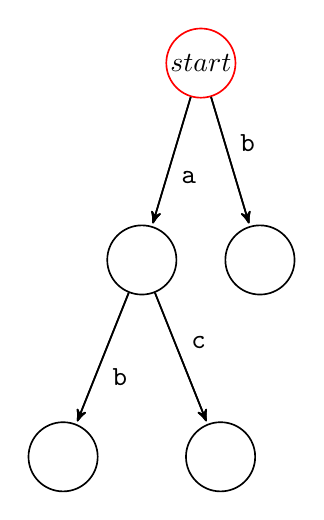
\begin{tikzpicture}[->,>=stealth',shorten >=1pt,auto,node distance=2.5cm, semithick]

% \node[rednode]           (ST)                    {$start$};
% \node[blacknode]         (A) [below left of=ST]  {};
% \node[blacknode]         (B) [below right of=ST] {};
% \node[blacknode]         (AB) [below left of=A]  {};
% \node[blacknode]         (AC) [below right of=A]    {};

\node[rednode](ST){$start$}
child{ node[blacknode](A){}
    child{node[blacknode] (AB){}}
    child{node[blacknode] (AC){}}
}
child{ node[blacknode](B){}}
;

\path
(ST) edge              node {\texttt{a}} (A)
     edge              node {\texttt{b}} (B)
(A)  edge              node {\texttt{b}} (AB)
     edge              node {\texttt{c}} (AC)
;
\end{tikzpicture}
\end{center}

其中红色节点代表起始状态,黑色节点代表结束状态。

\newpage

如何利用 Trie 树的结构,来求解配子生成函数,我们可以定义字符集 $\Sigma=\{\texttt{AA},\texttt{Aa},\texttt{aa},\texttt{BB},\texttt{Bb},\texttt{bb},\cdots\}$。

这是一棵插入了 $\texttt{AABb},\texttt{AABB},\texttt{AaBB},\texttt{AaBB}$ 的 Trie 树\footnote{我们在结束节点 $v$ 标记一个值 $cnt_v$,代表有多少字符串 $s$ 使得 $\delta(start,s)=v$。}。

\begin{center}
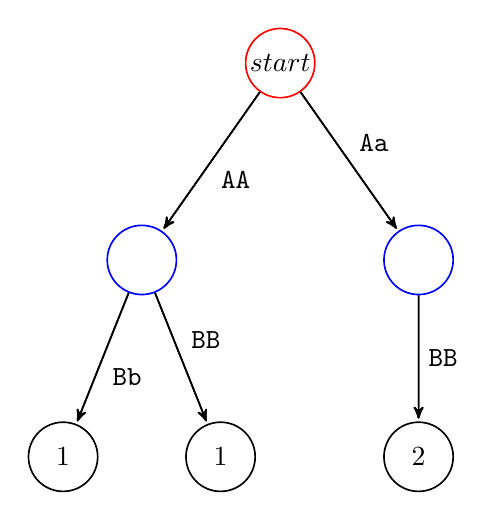
\begin{tikzpicture}[->,sibling distance=10em,>=stealth',shorten >=1pt,auto, semithick]

\node[rednode](ST){$start$}
child{ node[bluenode](AA){}
    child{node[blacknode] (AABb){1}}
    child{node[blacknode] (AABB){1}}
}
child{ node[bluenode](Aa){}
    child{node[blacknode] (AaBB){2}}
}
;

\path
(ST) edge              node {\texttt{AA}} (AA)
        edge              node {\texttt{Aa}} (Aa)
(AA) edge              node {\texttt{Bb}} (AABb)
        edge              node {\texttt{BB}} (AABB)
(Aa) edge              node {\texttt{BB}} (AaBB);
\end{tikzpicture}
\end{center}

程序实现时,我们从最底端开始递推,一直递推到第一层,我们的递推必须有\textsl{初状态}和\textsl{递推公式}。

我们首先来看初状态,节点 $v$ 的初状态就是 $cnt_v$,代表有多少种对应的基因型,为了便于理解,我们在图上节点旁标注初状态:

\begin{center}
\begin{tikzpicture}[->,sibling distance=10em,>=stealth',shorten >=1pt,auto, semithick]

\node[rednode](ST){$start$}
child{ node[bluenode](AA){}
    child{node[blacknode] (AABb){1}}
    child{node[blacknode] (AABB){1}}
}
child{ node[bluenode](Aa){}
    child{node[blacknode] (AaBB){2}}
}
;

\path
(ST) edge              node {\texttt{AA}} (AA)
     edge              node {\texttt{Aa}} (Aa)
(AA) edge              node {\texttt{Bb}} (AABb)
     edge              node {\texttt{BB}} (AABB)
(Aa) edge              node {\texttt{BB}} (AaBB);

\node[caption] at (AABb.south) {$1$};
\node[caption] at (AABB.south) {$1$};
\node[caption] at (AaBB.south) {$2$};

\end{tikzpicture}
\end{center}

我们再来看递推公式,设根节点的配子生成函数为 $F$,而它的三个子节点的配子生成函数为 $f_{\texttt{aa}},f_{\texttt{Aa}},f_{\texttt{AA}}$(如果不存在设为 $0$),那么有递推式:

$$
\begin{aligned}
    F &= (x^{\texttt{a}}+x^{\texttt{a}})f_{\texttt{aa}} + (x^{\texttt{A}}+x^{\texttt{a}})f_{\texttt{Aa}} + (x^{\texttt{A}}+x^{\texttt{A}})f_{\texttt{AA}} \\
      &= x^{\texttt{a}}(f_{\texttt{aa}} \times 2 + f_{\texttt{Aa}}) + x^{\texttt{A}}(f_{\texttt{AA}} \times 2 + f_{\texttt{Aa}})
\end{aligned}
$$

注意这里使用 $\texttt{Aa}$ 这对等位基因只是为了方便表述,事实上,这个递推式对任意一对等位基因都是成立的。

\newpage

有了初状态和递推公式,就可以通过程序递推到根节点,求解出整个种群的配子生成函数的和。

\textbf{递推到第二层}

\begin{center}
\begin{tikzpicture}[->,sibling distance=10em,>=stealth',shorten >=1pt,auto, semithick]

\node[rednode](ST){$start$}
child{ node[bluenode](AA){}
    child{node[blacknode] (AABb){1}}
    child{node[blacknode] (AABB){1}}
}
child{ node[bluenode](Aa){}
    child{node[blacknode] (AaBB){2}}
}
;

\path
(ST) edge              node {\texttt{AA}} (AA)
     edge              node {\texttt{Aa}} (Aa)
(AA) edge              node {\texttt{Bb}} (AABb)
     edge              node {\texttt{BB}} (AABB)
(Aa) edge              node {\texttt{BB}} (AaBB);

\node[caption] at (AABb.south) {$1$};
\node[caption] at (AABB.south) {$1$};
\node[caption] at (AaBB.south) {$2$};
\node at (AA.west) {$3x^{\texttt{B}}+x^{\texttt{b}} \qquad \qquad$};
\node at (Aa.east) {$\qquad 4x^{\texttt{B}}$};

\end{tikzpicture}
\end{center}

\textbf{递推到第一层}

$$\begin{aligned}F(x) &= x^{\texttt{A}}(2\times(3x^{\texttt{B}}+x^{\texttt{b}})+4x^{\texttt{B}})+x^{\texttt{a}}(4x^{\texttt{B}}) \\ &= 4x^{\texttt{aB}}+2x^{\texttt{Ab}}+10x^{\texttt{AB}}\end{aligned}$$

\begin{center}
\begin{tikzpicture}[->,sibling distance=10em,>=stealth',shorten >=1pt,auto, semithick]

\node[rednode](ST){$start$}
child{ node[bluenode](AA){}
    child{node[blacknode] (AABb){1}}
    child{node[blacknode] (AABB){1}}
}
child{ node[bluenode](Aa){}
    child{node[blacknode] (AaBB){2}}
}
;

\path
(ST) edge              node {\texttt{AA}} (AA)
     edge              node {\texttt{Aa}} (Aa)
(AA) edge              node {\texttt{Bb}} (AABb)
     edge              node {\texttt{BB}} (AABB)
(Aa) edge              node {\texttt{BB}} (AaBB);

\node[caption] at (AABb.south) {$1$};
\node[caption] at (AABB.south) {$1$};
\node[caption] at (AaBB.south) {$2$};
\node at (AA.west) {$3x^{\texttt{B}}+x^{\texttt{b}} \qquad \qquad$};
\node at (Aa.east) {$\qquad 4x^{\texttt{B}}$};
\end{tikzpicture}
\end{center}

\newpage

容易发现此做法的最坏时间复杂度为:

$$\mathcal T(i)=3 \times \mathcal T(i-1) + \mathcal O(2^i)$$

其中:

$$
\begin{aligned}
    \mathcal T(k) &= \mathcal O\left(\sum_{i=0}^k 2^i \times 3^{k-i} \right) \\
                  &= \mathcal O\left( \left (\sum_{i=0}^k (\frac{3}{2})^i \right) \times 2^k \right) \\
                  &= \mathcal O\left( \left(\frac{\left(\frac{3}{2}\right)^{k+1}-1}{\frac{3}{2}-1}\right) \times 2^k\right) \\
                  &= \mathcal O(3^{k+1} - 2^{k+1}) \\
                  &= \mathcal O(3^k-2^k)\\
                  &= \mathcal O(3^k)
\end{aligned}
$$

但是,通过严格的时间复杂度证明,可以发现这种做法一定比第一种做法要优,记 $n$ 为个体的个数,那么下界为 $\Omega(n)$,上界为 $\mathcal O(2^k)$。

实现时,我们可以考虑使用 \texttt{C++ Library} 中的 \texttt{vector} 数据结构,由于它按照元素个数倍增地开空间,可以获得较的空间复杂度。

\subsubsection{三种程序运行时间}

测评环境为 AMD EPYC 7K62 48-Core Processor。

\begin{table}[htbp]
	\centering
	\caption{当 $k=2,n=9$ 时的时间空间效率}
	\begin{tabular}{c|c|c|c}
		& $\texttt{solution0.cpp}$ & $\texttt{solution1.cpp}$ & $\texttt{solution2.cpp}$ \\ \hline
		时间 & 2ms & 2ms & 2ms \\ \hline
		空间 & 252KiB & 248KiB & 252KiB
	\end{tabular}
\end{table}

\begin{table}[htbp]
	\centering
	\caption{当 $k=15,n=15$ 时的时间空间效率}
	\begin{tabular}{c|c|c|c}
		& $\texttt{solution0.cpp}$ & $\texttt{solution1.cpp}$ & $\texttt{solution2.cpp}$ \\ \hline
		时间 & \color{red}{>1000ms} & 12ms & 10ms \\ \hline
		空间 & 1024KiB & 660KiB & 912KiB
	\end{tabular}
\end{table}

\begin{table}[htbp]
	\centering
	\caption{当 $k=13,n=531441$ 时的时间空间效率}
	\begin{tabular}{c|c|c|c}
		& $\texttt{solution0.cpp}$ & $\texttt{solution1.cpp}$ & $\texttt{solution2.cpp}$ \\ \hline
		时间 & \color{red}{>1000ms} & \color{red}{>1000ms} & 190ms \\ \hline
		空间 & 384KiB & 384KiB & 26432KiB
	\end{tabular}
\end{table}

\newpage

\subsection{基因片段生成函数的求法}

我们想求出一个基因片段生成函数乘法的快速实现。

\subsubsection*{朴素做法}

考虑朴素地实现 $(1)$ 中的卷积,时间复杂度为 $\mathcal O(4^k)$,是不能接受的。

\subsubsection*{优化的第一步}

我们发现 \textbf{对于只有显隐性情况的基因片段生成函数,可以转化为集合生成函数}。而且集合生成函数已经存在快速算法。

\subsubsection*{集合生成函数}

可以使用符号:

$$f=\sum_{S \subseteq U} f_S x^S$$

来表示一个\textsl{集合生成函数}。

这里我们定义算子 $\circ=\cup$,即:$x^L \times x^R=x^{L \cup R}$。

容易发现集合生成函数的乘法运算恰好为\textsl{集合并卷积},即:

$$h_S =\sum_{L} \sum_{R} [(L \cup R) = S] f_L g_R$$

\subsubsection*{基因片段生成函数到集合生成函数的转换}

定义全集 $U$ 是:$\{\texttt{A},\texttt{B},\cdots\}$。

我们将基因片段中的显性基因抽取出来,形成一个集合,如 $\texttt{ABc} \Rightarrow \{\texttt{A},\texttt{B}\}$。

这样发现集合并卷积刚好符合“显性基因克制隐形基因”的条件,因为只要某一位有对应的显性基因,那么个体就表现为显性,可以结合集合运算表来理解:

\begin{table}[htbp]
    \centering
    \caption{集合运算表}
    \begin{tabular}{cV{3}c|c}
        $\cup$ & $\{\texttt{A}\}$ & $\varnothing$ \\ \hlinewd{1pt}
        $\{\texttt{A}\}$ & $\{\texttt{A}\}$ & $\{\texttt{A}\}$\\ \hline
        $\varnothing$ & $\{\texttt{A}\}$ & $\varnothing$
    \end{tabular}
\end{table}


\subsubsection*{集合生成函数的快速卷积算法:FWT}

仿照 FFT 的思路,\textbf{我们求出 $f$ 的一种变换 $\hat f$,使得 $f * g = h \Rightarrow \hat f_i \times \hat g_i = \hat h_i$},即将系数表示法转化为点值表示法。

我们给出关于集合并卷积的 FWT 运算,即快速莫比乌斯变换。

$$\hat f_S=\sum_{T \subseteq S} f_T$$

证明:

$$
\begin{aligned}
    \hat h_S &=\sum_{L} \sum_{R} [(L \cup R) \subseteq S] f_L g_R \\
         &= \sum_{L} \sum_{R} [L \subseteq S][R \subseteq S] f_L g_R \\
         &= \sum_{L} [L \subseteq S] f_L \sum_{R} [R \subseteq S] g_R \\
         &= \hat f_S \hat g_S
\end{aligned}
$$

我们求出 $\hat h_S$ 后,当然需要将 $\hat h$ 转化为 $h$,于是需要反演运算:

$$f_S=\sum_{T \subseteq S} (-1)^{|S|-|T|}\hat f_T$$

由容斥原理可以证明。

\subsubsection*{朴素的变换和反演的实现}

枚举 $T$ 和 $S$,并且判断是否 $T \subseteq S$,时间复杂度 $\mathcal O(4^k)$,没有太大的变化。

\subsubsection*{经过优化的变换和反演的实现}

通过程序精细实现,能够以 $\mathcal O(2^{|S|})$ 的时间复杂度枚举 $S$ 的子集。

如果对于所有的 $S \subseteq U$,都这样枚举子集 $T$,时间复杂度为:

$$\mathcal O\left(\sum_{i=0}^k \binom{k}{i}2^i\right)= \mathcal O(3^k)$$

比朴素做法稍有进步。

\subsubsection*{进一步优化的变换和反演的实现}

我们使用递推的思路,推导出 $\hat f_S$。

设 $\hat f_S^{(i)}=\sum_{T\subseteq S}[(S\setminus T)\subseteq\{1,\cdots,i\}]f_T$,$\hat f_S^{(n)}$ 即是目标序列。

首先有 $\hat f_S^{(0)}=f_S$,因为只有当 $S \setminus T$ 为空集时,才能属于空集。

对于所有 $i\notin S$ 的 $S$,满足:

$$
\begin{cases}
\hat f_S^{(i)}=\hat f_S^{(i-1)} \\
\hat f_{S\cup\{i\}}^{(i)}=\hat f_S^{(i-1)}+\hat f_{S\cup\{i\}}^{(i-1)}
\end{cases}
$$

我们解释一下两个式子,对于第一个式子:

$$
\begin{aligned}
\hat f_S^{(i)} &= \sum_{T \subseteq S}[(S \setminus T)\subseteq\{1,\cdots,i\}]f_T\\
               &= \sum_{T \subseteq S}[(S \setminus T)\subseteq\{1,\cdots,i-1\}]f_T\\
               &= \hat f_S^{(i-1)}
\end{aligned}
$$

对于第二个式子:

$$
\begin{aligned}
\hat f_{S\cup\{i\}}^{(i)} &= \sum_{T \subseteq (S\cup\{i\})}[(S\cup\{i\}) \setminus T)\subseteq\{1,\cdots,i\}]f_T\\
               &= \sum_{T \subseteq (S\cup\{i\}) \text{ and } i \notin T}[((S\cup\{i\}) \setminus T)\subseteq\{1,\cdots,i\}]f_T+\sum_{T \subseteq (S\cup\{i\}) \text{ and } i \in T}[((S\cup\{i\}) \setminus T)\subseteq\{1,\cdots,i-1\}]f_T\\
               &= \sum_{T \subseteq S \text{ and } i \notin T}[(S \setminus T)\subseteq\{1,\cdots,i-1\}]f_T+\sum_{T \subseteq (S\cup\{i\}) \text{ and } i \in T}[((S\cup\{i\}) \setminus T)\subseteq\{1,\cdots,i-1\}]f_T\\
               &= \hat f_S^{(i-1)}+\hat f_{S \cup \{i\}}^{(i-1)}
\end{aligned}
$$

这样,我们 $\mathcal{O}(n2^n)$ 求出 $\hat f_S,\hat g_S$,按位乘,然后再反演回去即可。


\subsubsection*{快速莫比乌斯变换和反演的伪代码实现}

\begin{algorithm}
    \caption{快速莫比乌斯变换}
    \begin{algorithmic}[1]
        \Require 集合幂级数 $F$
        \Ensure $F$ 的莫比乌斯变换
        \Function {FastMobiusTransform}{$F$}
            \For{$i \gets 1 \textbf{ to } n$}
                \For{$\textbf{all }S \subseteq U \setminus \{i\}$}
                    \State $f_{S \cup \{i\}} \gets f_{S \cup \{i\}} + f_{S}$
                \EndFor
            \EndFor
            \State \Return{$F$}
        \EndFunction
    \end{algorithmic}
\end{algorithm}

\begin{algorithm}
    \caption{快速莫比乌斯反演}
    \begin{algorithmic}[1]
        \Require 集合幂级数 $F$
        \Ensure $f$ 的莫比乌斯反演
        \Function {FastMobiusInversion}{$F$}
            \For{$i \gets 1 \textbf{ to } n$}
                \For{$\textbf{all }S \subseteq U \setminus \{i\}$}
                    \State $f_{S \cup \{i\}} \gets f_{S \cup \{i\}} - f_{S}$
                \EndFor
            \EndFor
            \State \Return{$F$}
        \EndFunction
    \end{algorithmic}
\end{algorithm}

\newpage

\subsubsection*{求解表现型生成函数的伪代码实现}

\begin{algorithm}
    \caption{求解表现型生成函数}
    \begin{algorithmic}[1]
        \Require 配子生成函数 $G$
        \Ensure 表现型生成函数 $E$
		\Function {GetExpressionType}{$G$}
			\State G=FastMobiusTransform(G)
            \For{$\textbf{all }S \subseteq U$}
                \State $g_S=g_S \times g_S$
            \EndFor
			\State H=FastMobiusInversion(G)
            \State \Return{$H$}
        \EndFunction
    \end{algorithmic}
\end{algorithm}

\subsubsection*{此算法对于求解手算求解自由交配问题的启示}

\textbf{有两种基因型分别为 $\texttt{AaBb}$ 和 $\texttt{Aabb}$ 的个体,分别占比 $\frac{1}{3}$ 和 $\frac{2}{3}$,求解自由交配后的表现型比例。}

\begin{enumerate}
	\item 首先求解配子生成函数 $G$。\\ 
		$$
		\begin{aligned}
			G &= G_1+G_2 \\
			  &= \frac{1}{3} \times (\frac{1}{4}x^{\texttt{ab}}+\frac{1}{4}x^{\texttt{Ab}}+\frac{1}{4}x^{\texttt{aB}}+\frac{1}{4}x^{\texttt{AB}})+\frac{2}{3} \times (\frac{1}{2}x^{\texttt{ab}} + \frac{1}{2}x^{\texttt{Ab}}) \\
			  &= \frac{5}{12} x^{\texttt{ab}} + \frac{5}{12} x^{\texttt{Ab}} + \frac{1}{12} x^{\texttt{aB}} + \frac{1}{12} x^{\texttt{AB}}
		\end{aligned}
		$$
	\item 再转化为集合幂级数。\\
		$$F = \frac{5}{12} x^{\varnothing} + \frac{5}{12} x^{\{\texttt{A}\}} + \frac{1}{12} x^{\{\texttt{B}\}} + \frac{1}{12} x^{\{\texttt{A},\texttt{B}\}}$$
	\item 对它做莫比乌斯变换。\\
		$$
		\begin{aligned}
			\hat F &= \frac{5}{12} x^{\varnothing} + \frac{5+5}{12} x^{\{\texttt{A}\}} + \frac{1+5}{12} x^{\{\texttt{B}\}} + \frac{1+5+1+5}{12} x^{\{\texttt{A},\texttt{B}\}} \\
			  &= \frac{5}{12} x^{\varnothing} + \frac{10}{12} x^{\{\texttt{A}\}} + \frac{6}{12} x^{\{\texttt{B}\}} + \frac{12}{12} x^{\{\texttt{A},\texttt{B}\}}
		\end{aligned}
		$$
	\item 每一项都做平方。\\
		$$(\hat F)^2=\frac{25}{144} x^{\varnothing} + \frac{100}{144} x^{\{\texttt{A}\}} + \frac{36}{144} x^{\{\texttt{B}\}} + \frac{144}{144} x^{\{\texttt{A},\texttt{B}\}}$$
	\item 做莫比乌斯反演。\\
		$$
		\begin{aligned}
			F &= \frac{25}{144} x^{\varnothing} + \frac{100-25}{144} x^{\{\texttt{A}\}} + \frac{36-25}{144} x^{\{\texttt{B}\}} + \frac{144-100-36+25}{144} x^{\{\texttt{A},\texttt{B}\}} \\
			  &= \frac{25}{144} x^{\varnothing} + \frac{75}{144} x^{\{\texttt{A}\}} + \frac{11}{144} x^{\{\texttt{B}\}} + \frac{33}{144} x^{\{\texttt{A},\texttt{B}\}} \\
		\end{aligned}
		$$
	\item 即表现型比例 $\texttt{ab} : \texttt{Ab} : \texttt{aB} : \texttt{AB}=25:75:11:33$。
\end{enumerate}

\newpage

\section{只有显隐性情况群体自由交配的计算的推广}

\subsection{共显性问题}

有的时候一对等位基因对应的不只有一对相对性状,而有更复杂的情况。

例如有一种花卉,基因型为 $\texttt{AA}$ 时表现为红色,基因型为 $\texttt{Aa}$ 时表现为粉色,基因型为 $\texttt{aa}$ 时表现为白色。

\begin{table}[htbp]
    \centering
    \caption{共显性表现型表}
    \begin{tabular}{cV{3}c|c}
        $\operatorname{exp}$ & $\texttt{A}$ & $\texttt{a}$ \\ \hlinewd{1pt}
        $\texttt{A}$ & $\texttt{A}$ & $$\texttt{Aa}$$ \\ \hline
        $\texttt{a}$ & $\texttt{Aa}$ & $$\texttt{a}$$
    \end{tabular}
\end{table}

我们将基因片段中的显性和隐性基因抽取出来,形成一个集合,如 $\texttt{ABc} \Rightarrow \{\texttt{A},\texttt{B},\texttt{c}\}$,对这样的集合作集合并卷积,也可以理解为把一对等位基因拆成两位,$\texttt{A} \Rightarrow 10$,$\texttt{a} \Rightarrow 01$。

容易发现这样做的时间复杂度为 $\mathcal O(2k \times 2^{2k})=\mathcal O(2k \times 4^k)$,和朴素做法差不多,是不可接受的。

\subsection{复等位基因问题}

一对相对形状由多个等位基因决定.

例如 喷瓜的性别由等位基因 $\texttt{g}^{-},\texttt{g}^{+},\texttt{G}$ 决定,其中:

\begin{table}[htbp]
    \centering
    \caption{喷瓜表现型表}
    \begin{tabular}{cV{3}c|c|c}
        $\operatorname{exp}$ & $\texttt{g}^{-}$ & $\texttt{g}^{+}$ & $\texttt{G}$\\ \hlinewd{1pt}
        $\texttt{g}^{-}$ & $\texttt{g}^{-}$ & $\texttt{g}^{+}$ & $\texttt{G}$\\ \hline
        $\texttt{g}^{+}$ & $\texttt{g}^{+}$ & $\texttt{g}^{+}$ & $\texttt{G}$\\ \hline
        $\texttt{G}$ & $\texttt{G}$ & $\texttt{G}$ & $\texttt{G}$
    \end{tabular}
\end{table}

容易发现,这些等位基因构成一个\textsl{偏序集},我们发现若 $\texttt{g}^{-} \le \texttt{g}^{+} \le \texttt{G}$,则 $\operatorname{exp}$ 运算对应 $\max$ 运算。

将 $\texttt{g}^{-},\texttt{g}^{+},\texttt{G}$ 编码成为 $00,01,10$,那么容易看出:

\begin{table}[htbp]
    \centering
    \caption{编码运算表}
    \begin{tabular}{cV{3}c|c|c}
        $\operatorname{or}$ & $00(\texttt{g}^{-})$ & $01(\texttt{g}^{+})$ & $10(\texttt{G})$\\ \hlinewd{1pt}
        $00(\texttt{g}^{-})$ & $00(\texttt{g}^{-})$ & $01(\texttt{g}^{+})$ & $10(\texttt{G})$\\ \hline
        $01(\texttt{g}^{+})$ & $01(\texttt{g}^{+})$ & $01(\texttt{g}^{+})$ & $11(\texttt{G})$\\ \hline
        $10(\texttt{G})$ & $10(\texttt{G})$ & $11(\texttt{G})$ & $10(\texttt{G})$
    \end{tabular}
\end{table}

发现 $11,10$ 都对应 $\texttt{G}$,而 $00$ 对应 $\texttt{g}^-$,$01$ 对应 $\texttt{g}^+$。我们在程序实现时最后一步处理一下即可。

容易发现这样做的时间复杂度还是 $\mathcal O(2k \times 2^{2k})=\mathcal O(2k \times 4^k)$,和朴素做法差不多,是不可接受的。

\newpage

\section{集合卷积的进一步优化}

以上两个问题在只运用集合并卷积的情况下,都没有较低时间复杂度的算法,下面,我们引入高维 FWT,并且逐渐探寻 FWT 的一般式。

\subsection{定义}

定义生成函数 $F=\sum f_S x^S$,其中 $S$ 不再是一个集合,而是一个每维可以取 $0,\cdots ,k-1$ 的向量。

\subsection{每维取 max 的 FWT}

容易看出,当 $k=2$,而且:

$$\begin{aligned}0 \circ 0 = 0 \\ 1 \circ 0 = 1 \\ 0 \circ 1 = 1 \\ 1 \circ 1 = 1\end{aligned}$$

那么,这就对应了集合并卷积。

这里,我们不再讨论集合并卷积,而是考虑更加一般的形式,即 $\circ = \max$ 时的情形。

定义:

$$\hat f[x^S]=\sum[S \circ T=S] f_T$$

容易发现:

$$\hat h_S=\sum_{L}\sum_{R}[S \circ (L \circ R) = S] f_L \times g_R$$

由于:

$$\max(a,\max(b,c))=a \Leftrightarrow \max(a,b)=a \operatorname{and} \max(a,c)=a$$

有:

$$[(S \circ (L \circ R))=S]=[(S \circ L) =S][(S \circ R)=S]$$

得:

$$\begin{aligned} \hat h_S &= \sum_{L} \sum_{R} [(S \circ L) =S][(S \circ R)=S] f_L \times g_R \\ &= \sum_{L} [(S \circ L)=S] f_L \times \sum_{R} [(S \circ R)=S] g_R \\ &= \hat f_S \times \hat g_S\end{aligned}$$


那么,我们在 FWT 的 $k$ 个向量中,取前缀和即可,如果是反演的话,相邻做差即可。

\subsection{喷瓜问题的快速算法}

通过上述算法,将 $\texttt{g}^-$ 对应到 $0$,$\texttt{g}^+$ 对应到 $1$,$\texttt{G}$ 对应到 $2$,我们就可以解决上述的喷瓜问题,时间复杂度为 $\mathcal O(n \times 3^n)$。

\subsection{任意操作符的 FWT 问题}

容易发现,每次 FWT,都是在对其他位相同,而某一位分别为 $0, \cdots ,k-1$ 的 $k$ 个向量对应的下标做矩阵乘法。

如集合并卷积的矩阵:

$$\begin{bmatrix} 1 & 0 \\ 1 & 1 \end{bmatrix}$$

集合交卷积\footnote{运算符为 and 运算}的矩阵:

$$\begin{bmatrix} 1 & 1 \\ 0 & 1 \end{bmatrix}$$

集合对称差卷积\footnote{运算符为 xor 运算}的矩阵:

$$\begin{bmatrix} 1 & 1 \\ 1 & -1 \end{bmatrix}$$

上述 $\max$ 卷积的矩阵:

$$\begin{bmatrix} 1& 0 & 0& \cdots & 0\\ 1& 1& 0& \cdots & 0\\ 1& 1 & 1& \cdots & 0\\ \vdots& \vdots& \vdots& \ddots& \vdots\\ 1& 1& 1 & \cdots & 1 \end{bmatrix}$$

而反演则是乘对应的逆矩阵。

我们设矩阵为:

$$\mathbf{M}=\begin{bmatrix} a_{0,0}&  a_{0,1} &  a_{0,2}& \cdots &  a_{0,k-1}\\  a_{1,0}&  a_{1,1}&  a_{1,2}& \cdots &  a_{1,k-1}\\  a_{2,0}&  a_{2,1} &  a_{2,2}& \cdots &  a_{2,k-1}\\ \vdots& \vdots& \vdots& \ddots& \vdots\\  a_{k-1,0}&  a_{k-1,1}&  a_{k-1,2} & \cdots &  a_{k-1,k-1} \end{bmatrix}$$

由于 FWT 按位独立,对于某一维分析,有:

$$\left(\begin{bmatrix}f_0 \\ f_1 \\ f_2 \\ \vdots \\ f_{k-1} \end{bmatrix}\times \mathbf{M} \right) \cdot \left(\begin{bmatrix}g_0 \\ g_1 \\ g_2 \\ \vdots \\ g_{k-1} \end{bmatrix}\times \mathbf{M}\right) = \begin{bmatrix}h_0 \\ h_1 \\ h_2 \\ \vdots \\ h_{k-1} \end{bmatrix}\times \mathbf{M}$$

其中 $\cdot$ 代表“按位乘”,即:

$$\begin{bmatrix}f_0 \\ f_1 \\ f_2 \\ \vdots \\ f_{k-1} \end{bmatrix} \cdot \begin{bmatrix}g_0 \\ g_1 \\ g_2 \\ \vdots \\ g_{k-1} \end{bmatrix} = \begin{bmatrix}f_0 \times g_0 \\ f_1 \times g_1 \\ f_2 \times g_2 \\ \vdots \\ f_{k-1} \times g_{k-1} \end{bmatrix}$$

由于 $h_{i}=\sum_{j,k} [j \circ k =i]f_{j} \times g_{k}$,枚举每个 $i$,对于每个 $f_j \times g_k$ 分析,容易列出方程:

$$a_{i,j} \times a_{i,k}=a_{i,j \circ k}$$

发现不管对于哪个 $i$,方程都是一样的,去掉 $i$,我们就只用解方程 $a_{j} \times a_{k}=a_{j \circ k}$。

如,当 $\circ$ 运算为取 $\operatorname{or}$ 的时候,有:

$$
\begin{cases}
    a_{0} \times a_{0}=a_{0} \\
    a_{1} \times a_{0}=a_{1} \\
    a_{0} \times a_{1}=a_{1} \\
    a_{1} \times a_{1}=a_{1} \\
\end{cases}
$$

我们解出两组解:

$$
\begin{aligned}
    \begin{cases}
        a_{0} =1 \\
        a_{1} =0 \\
    \end{cases}
    \qquad
    \begin{cases}
        a_{0} =1 \\
        a_{1} =1 \\
    \end{cases}
\end{aligned}
$$

于是可以这样安排我们的矩阵:

$$\mathbf{M}_1=\begin{bmatrix} 1 & 0 \\ 1 & 1 \end{bmatrix}$$

$$\mathbf{M}_2=\begin{bmatrix} 1 & 1 \\ 1 & 0 \end{bmatrix}$$

为什么不能这样这样安排:

$$\mathbf{M}_3=\begin{bmatrix} 1 & 0 \\ 1 & 0 \end{bmatrix}$$

$$\mathbf{M}_4=\begin{bmatrix} 1 & 1 \\ 1 & 1 \end{bmatrix}$$

原因是,这两个矩阵都没有对应的逆矩阵,求逆矩阵可以再列出一个方程,然后解出 $x_0,x_1$。(可以注意到求解方程的意义正好对应了 FWT 逆操作的意义)

$$
\begin{cases}
    a_{0,0}x_0 + a_{0,1}x_1 =b_0 \\
    a_{1,0}x_0 + a_{1,1}x_1 =b_1 \\
\end{cases}
$$

拿 $\mathbf{M}_1$ 举例,有:

$$
\begin{cases}
    x_0 = b_1 \\
    x_0 + x_1 =b_2 \\
\end{cases}
$$

那么显然:

$$
\begin{cases}
    x_0 = b_1 \\
    x_1 = b_2-b_1 \\
\end{cases}
$$

于是其逆矩阵就是:

$$\mathbf{M}_1^{-1}=\begin{bmatrix} 1 & 0 \\ -1 & 1 \end{bmatrix}$$

而对于 $\mathbf{M}_3$ 来说,有:

$$
\begin{cases}
    x_0 = b_1 \\
    x_0 = b_2 \\
\end{cases}
$$

显然不合法。于是不能使用 $\mathbf{M}_3$ 这个矩阵。

这样,我们解出矩阵 $\mathbf{M}$,然后求出逆矩阵 $\mathbf{M}^{-1}$,就可以解决任意操作符 $\circ$ 的 FWT 问题。

\subsection{$\circ$ 运算需要满足的性质}

由于:

$$a_{j} \times a_{k}=a_{j \circ k}$$

有:

$$
a_{j \circ k}=a_j \times a_k=a_k \times a_j=a_{k \circ j}
$$

$$
a_{j \circ (k \circ l)}=a_j \times a_{k \circ l}=a_j \times a_k \times a_l=a_{j \circ k} \times a_{l}=a_{(j \circ k)\circ l}
$$

于是 $\circ$ 运算必须满足交换律和结合律。

\subsection{不进位加法的 FWT}

我们定义不进位加法 $\oplus_p$ 运算,为:

$$
a \oplus_p b  =
\left\{
    \begin{array}{l}
        a+b \quad (0 \le a+b \le p-1) \\
        a+b-p \quad (p \le a+b \le 2p-2) \\
    \end{array}
\right.
$$

容易发现,其矩阵系数 $a$ 满足:

$$a_{i,j} \times a_{i,k}=a_{i,j \oplus_p k}$$

这里,我们发现,这组方程的特解即是:

$$a_{i,j} = \omega_{p}^j$$

因为单位根运算满足:

$$\omega_{p}^k = \omega_{p}^{k+p}$$

$$\omega_{p}^{i+j} = \omega_{p}^i \times \omega_{p}^j$$

进而发现,方程有 $p$ 组解,第 $i$ 组解(从 $0$ 开始编号)为:

$$a_{i,j} = \omega_{p}^{j \times i}$$

那么我们可以列出矩阵:

$$
\begin{bmatrix} 1& 1 & 1& \cdots & 1\\ 1& \omega_p^1& \omega_p^2& \cdots & \omega_p^{p - 1}\\ 1& \omega_p^2 & \omega_p^4& \cdots & w_p^{2(p - 1)}\\ \vdots& \vdots& \vdots& \ddots& \vdots\\ 1& \omega_p^{p - 1}& \omega_p^{2(p - 1)} & \cdots & \omega_p^{(p - 1)(p - 1)} \end{bmatrix}
$$

此矩阵就是\textsl{范德蒙德矩阵}。

我们不加证明地给出它的逆矩阵:

$$
\frac 1 p \begin{bmatrix} 1& 1 & 1& \cdots & 1\\ 1& \omega_p^{-1}& \omega_p^{-2}& \cdots & \omega_p^{-(p - 1)}\\ 1& \omega_p^{-2} & \omega_p^{-4}& \cdots & \omega_p^{-2(p - 1)}\\ \vdots& \vdots& \vdots& \ddots& \vdots\\ 1& \omega_p^{-(p - 1)}& \omega_p^{-2(p - 1)} & \cdots & \omega_p^{-(p - 1)(p - 1)} \end{bmatrix}
$$

这样,我们就可以完成模 $p$ 意义下的不进位加法卷积,此算法即\textsl{多维广义离散傅里叶变换}。

具体程序实现,我们可以算出 $\omega_p^1$ 即 $\cos \frac{p}{2\pi} + i\sin \frac{p}{2\pi}$,如果能用根号形式表示,即:$a+b\sqrt{x}i$,我们可以模拟复数 $a+b\sqrt{x}i$,其乘法为 $(a+b\sqrt{x}i)(c+d\sqrt{x}i)=(ac-xbd)+(ac+bd)\sqrt{x}i$,加法为 $(a+b\sqrt xi)+(c+d\sqrt xi)=(a+b)+(c+d)\sqrt xi$。

或者,更加通用地,我们将长度为 $p$ 的多项式环作为一种数据结构,假设是 $F=\sum_{i=0}^{p-1} \omega_p^i f_i$,有:$F \times \omega_p^k=F=\sum_{i=0}^{p-1} \omega_p^i f_{i\ominus k}$,$F \times G=\sum_{i=0}^{p-1} \sum_{j=0}^{p-1} w_p^{i \oplus j} f_i \times g_j$。

此算法也可以使用 Bluestein's Algorithm 优化,即对上式变形后再进行一次卷积:

$$
\begin{aligned}
	[x^k]F & = \sum_{i=0}^{n-1}f_i\omega_n^{ik} \\
	& = \sum_{i=0}^{n-1}f_i\omega_{2n}^{-{(k-i)^2+i^2+k^2}} \\
	& = \omega_{2n}^{-{k^2}}\sum_{i=0}^{n-1}f_i\omega_{2n}^{-{i^2}}\omega_{2n}^{-{(k-i)^2}}
\end{aligned}
$$

但是通常 $k$ 不大,所以和直接暴力卷积时间上差距会不大。

\begin{algorithm}
    \caption{多维广义离散傅里叶变换}
    \begin{algorithmic}[1]
        \Require 幂级数 $f$,单位根 $w_p$,操作符 $opr$ 代表正变换还是逆变换。
        \Ensure $f$ 的傅里叶变换
        \Function {FourierTransform}{$f,w_p,opr$}
            \If $\ opr=1$
                \State $\textbf{M}_{i,j} \gets w^{(i-1)(j-1)}_p$
            \Else
                \State $\textbf{M}_{i,j} \gets \frac{1}{p}w^{-(i-1)(j-1)}_p$
            \EndIf
            \For{$i \gets 1 \textbf{ to } n$}
                \For{$\texttt{p vectors satisfying }1 \cdots p\texttt{ on the i-th bit and the other bits are same.}$}
                    \State $v \gets \texttt{the p vectors}$
                    \For{$j \gets 1 \textbf{ to } p$}
                        \State $g_j \gets f_{v_j}$
                    \EndFor
                    \State $g \gets g \times \textbf{M}$
                    \For{$j \gets 1 \textbf{ to } p$}
                        \State $f_{v_j} \gets g_j$
                    \EndFor
                \EndFor
            \EndFor
            \State \Return{$f$}
        \EndFunction
    \end{algorithmic}
\end{algorithm}

\subsection{共显性问题的快速算法}

如果将 $\texttt{A}$ 对应到 $1$,$\texttt{a}$ 对应到 $0$,容易发现:

\begin{table}[htbp]
    \centering
    \caption{编码运算表}
    \begin{tabular}{cV{3}c|c}
        $+$ & $1(\texttt{A})$ & $0(\texttt{a})$\\ \hlinewd{1pt}
        $1(\texttt{A})$ & $2(\texttt{A})$ & $1(\texttt{Aa})$\\ \hline
        $0(\texttt{a})$ & $1(\texttt{Aa})$ & $0(\texttt{a})$\\
    \end{tabular}
\end{table}

我们发现 $\texttt{A}$ 对应 $2$,$\texttt{Aa}$ 对应 $1$,$\texttt{a}$ 对应 $0$。

只要使用三次单位根 $\omega_3=\cos 120^\circ + \rm i \sin 120^\circ$,即可轻松解决此问题,时间复杂度是 $\mathcal O(n \times 3^n)$。

\newpage

\section{通过后代表现型生成函数倒推亲代配子生成函数}

在生产生活中,有时并不能知道亲代的基因型,这时,我们可以使用上述算法的逆操作,先将表现型生成函数做一次 FWT,之后开根号,最后再 FWT 回去:

\begin{algorithm}
	\caption{求解亲代配子生成函数}
	\begin{algorithmic}[1]
		\Require 表现型生成函数 $E$
		\Ensure 配子生成函数 $G$
		\Function {GetGameteType}{$E$}
		\State E=FastMobiusTransform(E)
		\For{$\textbf{all }S \subseteq U$}
		\State $e_S=\sqrt{e_S}$
		\EndFor
		\State G=FastMobiusInversion(E)
		\State \Return{$E$}
		\EndFunction
	\end{algorithmic}
\end{algorithm}

事实上,得知亲代配子生成函数,并不能推出亲代个体基因型生成函数,因为可能存在多对一的情况,如 $\frac{1}{2}x^{\texttt{AA}}+\frac{1}{2}x^{\texttt{aa}}$ 和 $x^{\texttt{Aa}}$ 对应的配子生成函数都是一样的。但是在研究生物的进化时,配子生成函数远比个体基因型生成函数有用得多。

\section{多倍体的解法}

多倍体是指体细胞中含有三个或三个以上染色体组的个体,为了方便起见,以下我们都讨论三倍体。

容易发现,三倍体进行配子生成函数的运算时,需要乘三次,于是针对只有显隐性情况的群体自由交配,我们可以设计以下的算法:

\begin{algorithm}
	\caption{求解多倍体表现型生成函数}
	\begin{algorithmic}[1]
		\Require 配子生成函数 $G$
		\Ensure 表现型生成函数 $E$
		\Function {GetPolyploidExpressionType}{$G$}
		\State G=FastMobiusTransform(G)
		\For{$\textbf{all }S \subseteq U$}
		\State $g_S=g_S \times g_S \times g_S$
		\EndFor
		\State H=FastMobiusInversion(G)
		\State \Return{$H$}
		\EndFunction
	\end{algorithmic}
\end{algorithm}

这样的算法还可以推广到更多的情况,这里不再赘述。

\section{非等位基因之间的常见相互作用以及对应的解法}

\subsection{互补基因(Complementary gene)}

若干个非等位的显性基因只有同时存在时才出现某一性状,其中任何一个基因发生突变都会导致同一突变型性状,这些基因称为互补基因。

我们可以使用集合并卷积,不同的是只要配子有两个基因其中一个时,该位就为 1。

\subsection{累加作用(Additive effect)}

两种显性基因同时存在时表现为一种性状;单独存在时,表现另一种性状;而两对基因均为隐性纯合时表现第三种性状。

发生累加作用的每个基因只有部分作用。

我们可以使用不进位加法卷积,当这个基因对某种性状有增加作用时,记为 $+1$,而有减少作用是则记为 $-1$,最后对每个配子都这么算一遍再卷积。

事实上,上述共显性问题是累加作用的一个子集。

\subsection{抑制作用(Inhibitor)和上位效应(Epistasis)}

有些基因本身并不能表现任何可见的表型效应,但它的存在,完全抑制了其它非等位基因的作用,这种基因称为抑制基因。

两对独立遗传的基因共同对某一性状发生作用,而且其中一对基因对另一对基因的表现有遮盖作用,这种效应称为上位效应。

我们可以使用取 $\max$ 的卷积,对于抑制基因,可以将其设为极大值,而上位基因的隐性基因设为极小值,显性基因设为极大值。

\subsection{总结一般规律}
在这里,我们使用了化归的思想,将未知的问题转化为我们已知的不进位加法卷积和取 $\max$ 的卷积,从而获得了具有普适性的解法。同时,需要强调的是,只要基因之间的相互作用具有“抑制”的意义,就可以使用取 $\max$ 的卷积,而基因之间的相互作用具有“叠加”的意义,就可以使用不进位加法卷积。s

\section{纯合致死问题的快速算法}

生物界中,有一些个体会因为显性基因纯合而死亡,我们假定有 $k$ 对等位基因,只要其中一对显性纯合,个体都会胚胎致死,通过共显性问题的快速做法,我们可以得到一个时间复杂度为 $\mathcal O(n \times 3^n)$ 的做法,但是这个时间复杂度有些过大。

为了研究这类问题的快速做法,我们引入 \textsl{子集卷积}。

\subsection{子集卷积}

定义:

$$h_S =\sum_{L} \sum_{R} [(L \cup R) = S][(L \cap R)=\varnothing] f_L g_R$$

为集合幂级数 $F$ 和 $G$ 的子集卷积。

\subsection{子集卷积的朴素实现}

用我们之前提到过的枚举子集方法,可以 $\mathcal O(3^k)$ 实现子集卷积,参见 \texttt{solution0.cpp}。该做法已经比上述做法优秀了,但是我们还要寻求更加优秀的做法。

\subsection{子集卷积的快速实现}

注意到:$[L\cup R=S][L\cap R=\varnothing]=[L\cup R=S][|L|+|R|=|S|]$。

定义二元幂级数 $\mathbf f_{i,S}$,$\mathbf f_{|S|,S}=f_{S}$,其他情况均为 $0$。

式子可化为:

$$\mathbf h_{i,S}=\sum_{L\subseteq U} \sum_{R\subseteq U} [L \cup R=S][i=j+k] \mathbf f_{j,L} \mathbf g_{k,R}$$

那么就可以把它看成二元生成函数,第一维就是普通卷积,第二维是集合卷积。我们处理这类问题的方法是分别对两维做卷积,可以参照 \texttt{solution1.cpp}。

\subsection{实际效率}

通过 \texttt{\_\_int128} 等优化,发现有时朴素做法时间上比快速做法还优秀。

\begin{table}[htbp]
	\centering
	\caption{当 $k=17$ 时的时间空间效率}
	\begin{tabular}{c|c|c}
		& $\texttt{solution0.cpp}$ & $\texttt{solution1.cpp}$\\ \hline
		时间 & 194ms & 245ms \\ \hline
		空间 & 3240KiB & 59628 KiB 
	\end{tabular}
\end{table}

当内存比较紧张时,朴素做法也是一种可以考虑的做法。

\section{不允许自交时的计算方法}

当不允许自交时,可以使用类似于我们使用 Trie 树求配子的方法,然后去掉不合法的方案。

\section{多不同作用等位基因时的优化}

由于 FWT 按位独立,我们可以使用类似于康托展开的做法,来获得一个较为密集的编号。

假设现在有一个 $k$ 为向量 $\vec F$,第 $i$ 维能够取到的值有 $S_{i,1},S_{i,2},\cdots,S_{i,|S_i|}$。那么,我们使用这样的编号方法:

$$\vec F \to \sum_{i=1}^k \sum_{j=1}^{|S_i|} [\vec F_i = S_{i,|S_i|}](\prod_{j=1}^{i-1}|S_j|)$$

就可以获得时间复杂度为 $\mathcal O(k\prod_{i=1}^k |S_i|)$ 的做法。

\section{蓝色玫瑰问题}

\subsection{问题描述}

你有一张表,记录了基因型对应的花色,你一开始有某些种基因型对应的种子,在花朵未开放之前,你可以挑选花朵的颜色,保留一些想要的颜色,而去除不想要的颜色。然后剩下的花开放后自由交配(可以自交)。求最少培育多少株植物,才能得到想要的蓝色花色。你只能使用当前代系玫瑰的种子,而不能使用前面几代的花种,因为它们已经过期了。

\subsection{思路与方法}

容易发现,该问题中,能够掌握的仅是挑选哪些颜色。我们希望通过程序,做出最优化的选择。这就让我们想到了对每个颜色做出“估价”,然后问题转化为了挑选一些颜色,使得估价最大化。

\subsection{对配子的估价}

首先,我们需要对配子做出估价,我们容易想到如下的几个估价函数:

$$g_1(\vec G)=\sum_{[color(\vec F)=blue]} \sum_{i=1}^k ([\vec G_i=\vec F_{i,0}]+[\vec G_i=\vec F_{i,1}])$$

$$g_2(\vec G)=2^{g_1(\vec G)}$$

$$g_3(\vec G)=\sum_{[color(\vec F)=blue]} \sum_{i=1}^k ([\vec G_i=\vec F_{i,0} \text{ and } \vec G_i=\vec F_{i,1}])$$

\subsection{对颜色的估价}

对颜色的估价,实际就是该颜色对应的基因型产生的配子估价值的总和。

$$g(c)=\sum_{[color(\vec F)=c]} \sum_{\vec G \in G(\vec F)} g(\vec G)$$

\subsection{最优化的策略}

我们不能选取全部颜色,而是只能选取部分颜色,因为不能培养太多种子,我们再定义函数 $cnt(c)=\sum_F [color(\vec F)=c]$,代表颜色 $c$ 对应了多少个体,那么我们需要以下的值最大:

$$M=\frac{\sum_{c \in S} g(c)}{\sum_{c\in S}{cnt(c)}}$$

事实上这是一个 01 分数规划问题,通过 $\mathcal O(n \log |S|)$ 的二分,就可以求出答案。

\newpage

\bibliographystyle{unsrt} %按照引用顺序排序
\bibliography{mybib} %bib文件的文件名

\end{document}